
\section{Load Balancing Challenges in VLM RL Training}
\label{sec:background}

\subsection{Data Preparation Bottleneck}

\begin{wrapfigure}{r}{0.25\textwidth}
    \vspace{-10pt}
    \centering
    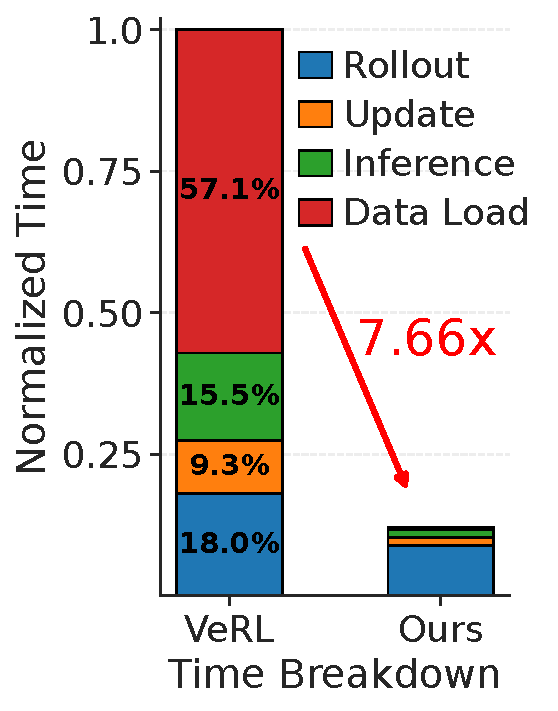
\includegraphics[width=\linewidth]{figures/time_breakdown_ablation_20260228_201525.pdf}
    \vspace{-12pt}
    \caption{Iteration time breakdown of GRPO.}
    \label{fig:time_breakdown}
    \vspace{-10pt}
\end{wrapfigure}

% Unlike text-only RL, multimodal RL must repeatedly fetch and preprocess large visual payloads (e.g., decoding video clips and sampling frames) on the critical path. Many RL frameworks, such as veRL~\citep{verl}, adopt a hybrid-controller architecture that centralizes these CPU- and I/O-heavy operations on a single master node, which then dispatches materialized tensors to workers. As the global batch size grows, the master’s preprocessing time and host-memory footprint scale with the amount of visual data, quickly turning it into the pipeline straggler and frequently triggering CPU out-of-memory (OOM) errors. Figure~\ref{fig:time_breakdown} illustrates this effect: in veRL, data loading accounts for 57.1\% of the step time, exceeding rollout (18.0\%), inference (15.5\%), and update (9.3\%) combined. This motivates a distributed, metadata-driven data pipeline (ShadowLoader; Sec.~\ref{sec:shadowloader}) that parallelizes preprocessing and hides data movement behind GPU computation.

Unlike text-only RL, multimodal RL must repeatedly fetch and preprocess large visual payloads (e.g., decoding video clips and sampling frames). Existing RL frameworks often rely on centralized controller to orchestrate distributed rollout, inference and training. They centralize the CPU- and I/O-heavy operations on the driver node, which also dispatches materialized tensors to workers.  In a veRL multimodal baseline, we observe that visual data loading, preprocessing, and dispatch remain concentrated in the centralized controller, which exposes huge bubbles on the critical path and causes CPU I/O stragglers and large host-memory pressure as the global batch size increases. Figure~\ref{fig:time_breakdown} illustrates this effect: in our veRL baseline, data loading accounts for 57.1\% of the step time, exceeding rollout, inference, and update combined. This motivates a distributed, metadata-driven data pipeline that parallelizes preprocessing and overlaps data movement with GPU computation.


\subsection{Compute and Memory Imbalance in Model Execution}

Beyond data loading, the execution phase suffers from severe compute and memory imbalances. First, attention computation scales quadratically with sequence length, while activation memory scales linearly. A placement strategy that equalizes memory across GPUs can still result in severe compute imbalance, and vice versa. Second, multimodality introduces heterogeneous costs that are poorly correlated with text length. The computational cost of the vision tower depends heavily on the number of images or video frames. Mixing video-heavy and image-heavy samples within the same batch creates massive variance in per-sample compute and memory requirements, making length-only bucketing objectives ineffective.

\subsection{Why Existing Load Balancing Falls Short in VLM RL}

\noindent\textbf{Fixed-parallelism bucketing/packing.}~Classic bucketing methods~\citep{KimiVL,KeyeVL,InternVL3_5,GLM-4_5V} sort sequences by length and pack them into per-GPU buckets under a fixed parallelism configuration. While simple, this strategy fails when a single long outlier dominates the step. For instance, as shown in Figure~\ref{fig:motivation}(Middle), with sequences of varying lengths (e.g., 32K, 16K, and 4K) on four GPUs, no matter how sequences are bucketed, the GPU processing the 32K sample becomes the bottleneck, leading to unavoidable slowdowns. This issue persists in 3D/4D parallelism settings that assume homogeneous configurations across DP ranks.

\noindent\textbf{Heterogeneous DP across buckets.}~Methods such as FlexSP~\citep{FlexSP}, HotSPa~\citep{HotSPa}, Hydraulis~\citep{Hydraulis}, and ByteScale~\citep{ByteScale} assign different parallelism configurations to different buckets. However, they rely on large batch sizes and gradient accumulation to create sufficient scheduling space for sequence reordering. This assumption is not always satisfied in RL settings: frequent rollout-update alternations can leave limited room for aggregation, especially when the effective batch size is modest or when only a few gradient steps are taken between rollouts. In such cases, re-sharding, extra synchronization, and optimizer-state movement can become prohibitively expensive. Furthermore, when sequence parallelism (SP) is enabled, short sequences suffer from redundant communication overhead, and assigning a single SP degree per bucket fails to accommodate mixed-length samples.

% \noindent\textbf{Length-only objectives ignore multimodal heterogeneity.}~Bucketing by text length alone fails to capture the vision-tower workload. Mixing videos and images within a bucket yields highly skewed per-GPU compute and memory footprints, even if the total token counts appear balanced.

% Together, these limitations motivate a finer-grained, modality-aware load-balancing mechanism capable of balancing both compute and memory under small-batch RL constraints, which we introduce in Sec.~\ref{sec:system_design}.

\begin{figure}
    \centering
    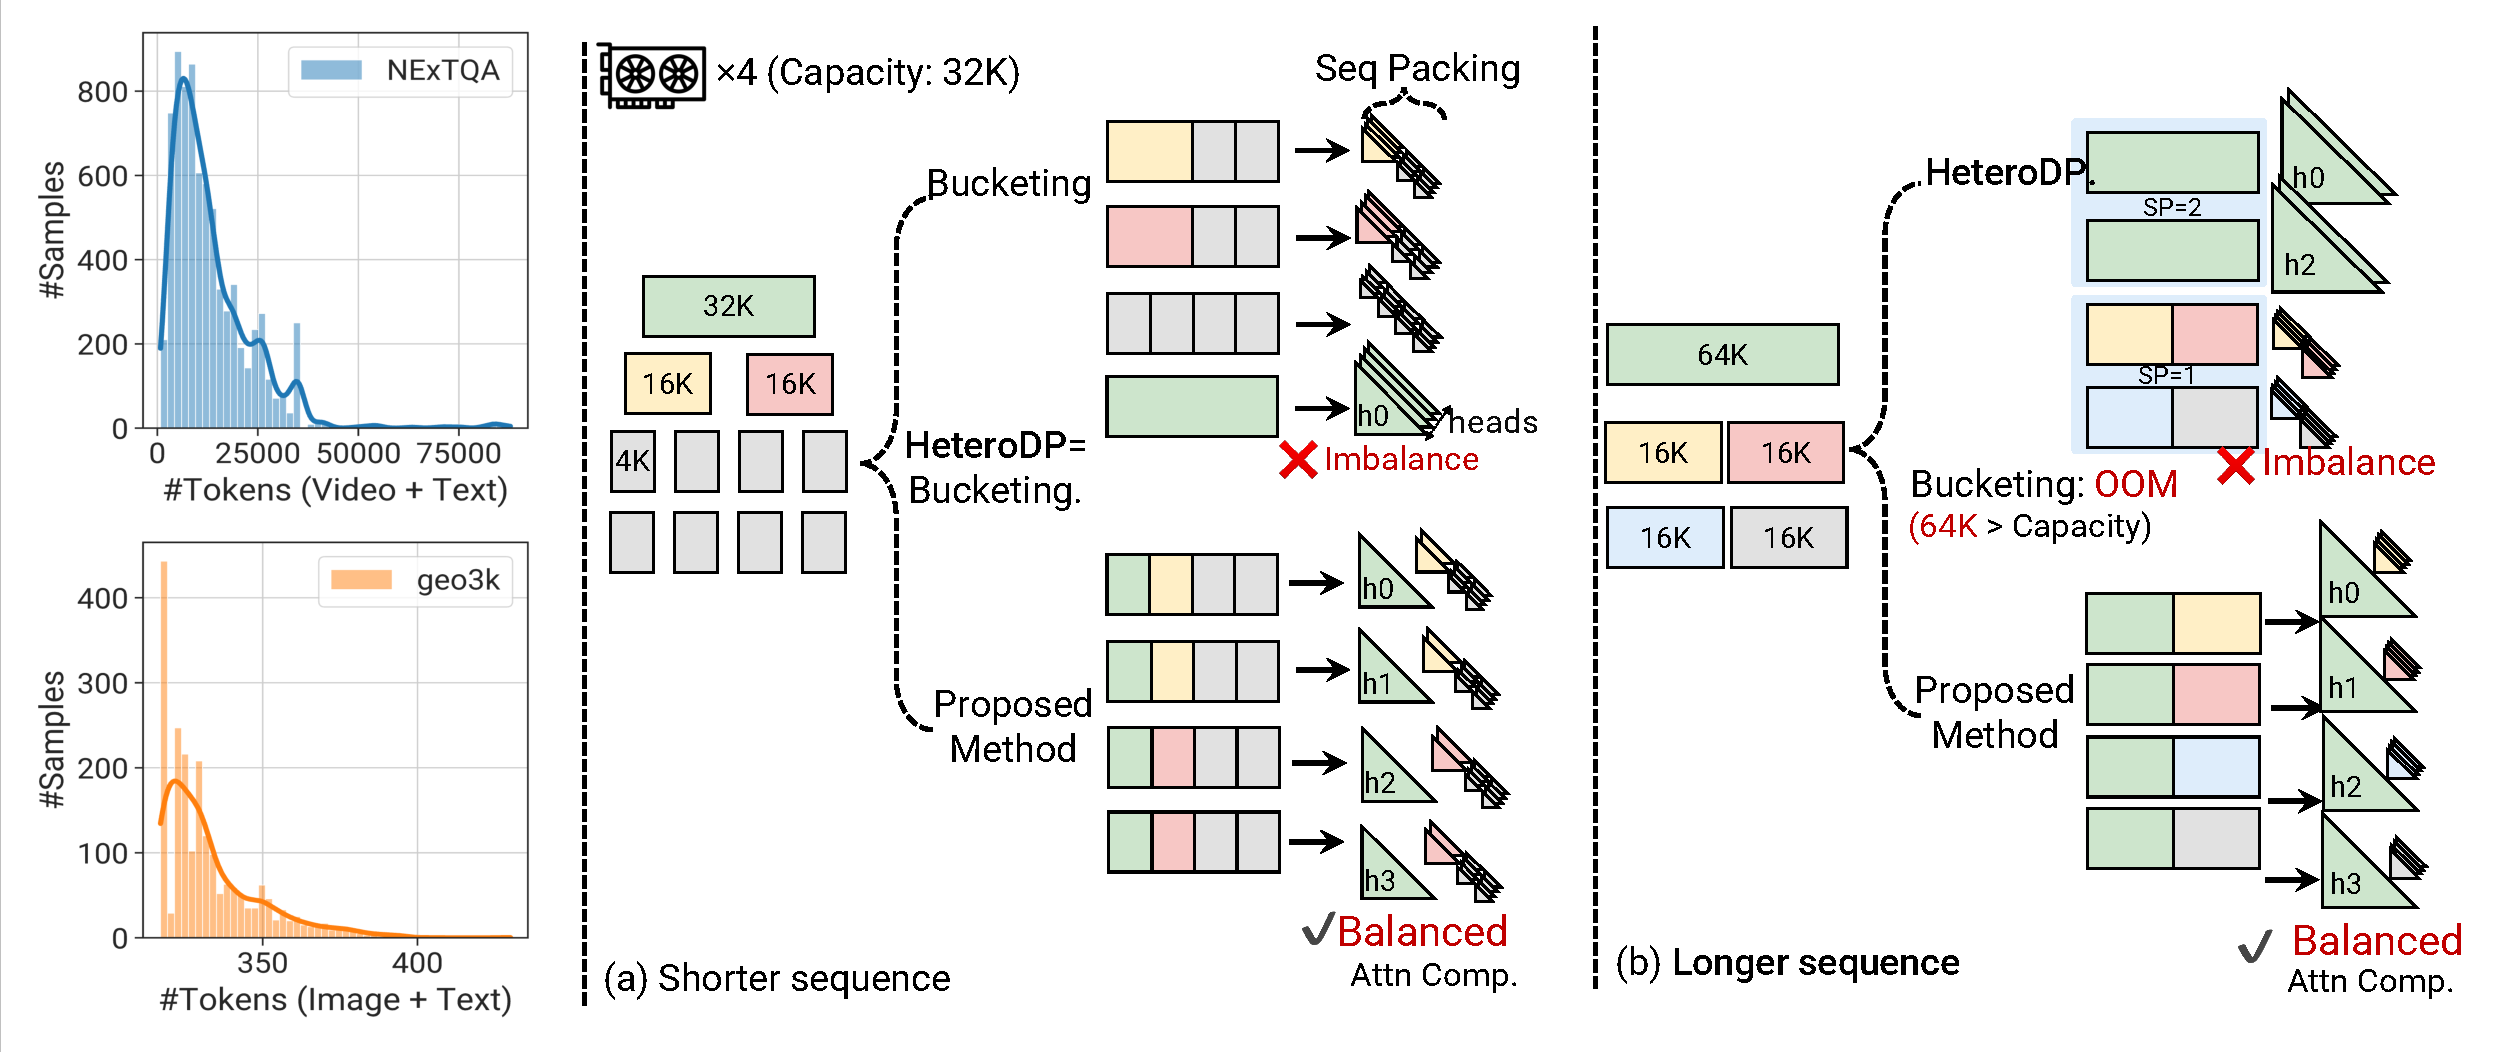
\includegraphics[width=0.95\textwidth]{figures/imbalance.pdf}
    \caption{Motivation and idea of FlexUlysses. \textbf{Left}: Distribution of token counts in typical video-text (NExTQA~\citep{nextqa}) and image-text (Geo3K\citep{geo3k}) datasets, showing extreme variation in sequence lengths. \textbf{Middle}: An imbalance with shorter sequences, where conventional bucketing leads to load imbalance. \textbf{Right}: For longer sequences, bucketing can cause out-of-memory (OOM) errors and further imbalance, while our approach enables fine-grained sharding and balanced attention computation across GPUs.}
    \label{fig:motivation}
\end{figure}
